\documentclass[a4paper,12pt,oneside]{book}

%-------------------------------Start of the Preable------------------------------------------------
\usepackage[english]{babel}
\usepackage{blindtext}

%packagr for hyperlinks
\usepackage{hyperref}
\hypersetup{
    colorlinks=true,
    linkcolor=blue,
    filecolor=magenta,      
    urlcolor=cyan,
}

\urlstyle{same}
%use of package fancy header
\usepackage{fancyhdr}
\usepackage{subcaption}
\renewcommand{\arraystretch}{1}
\usepackage{tabulary}
\usepackage[newcommands]{ragged2e}

\setlength\headheight{26pt}
\fancyhf{}
%\rhead{
\includegraphics[width=1cm]{logo}}
\lhead{\rightmark}
\rhead{
\includegraphics[width=1cm]{logo}}
\fancyfoot[RE, RO]{\thepage}
\fancyfoot[CE, CO]{\href{http://www.e-yantra.org}{www.e-yantra.org}}

\pagestyle{fancy}

%use of package for section title formatting
\usepackage{titlesec}
\titleformat{\chapter}
  {\Large\bfseries} % format
  {}                % label
  {0pt}             % sep
  {\huge}           % before-code
 
%use of package tcolorbox for colorful textbox
\usepackage[most]{tcolorbox}
\tcbset{colback=cyan!5!white,colframe=cyan!75!black,halign title = flush center}

\newtcolorbox{mybox}[1]{colback=cyan!5!white,
colframe=cyan!75!black,fonttitle=\bfseries,
title=\textbf{\Large{#1}}}

%use of package marginnote for notes in margin
\usepackage{marginnote}

%use of packgage watermark for pages
%\usepackage{draftwatermark}
%\SetWatermarkText{
\includegraphics{logo}}
\usepackage[scale=2,opacity=0.1,angle=0]{background}
\backgroundsetup{
contents={
\includegraphics{logo}}
}

%use of newcommand for keywords color
\usepackage{xcolor}
\newcommand{\keyword}[1]{\textcolor{red}{\textbf{#1}}}

%package for inserting pictures
\usepackage{graphicx}

%package for highlighting
\usepackage{color,soul}

%new command for table
\newcommand{\head}[1]{\textnormal{\textbf{#1}}}


%----------------------End of the Preamble---------------------------------------


\begin{document}

%---------------------Title Page------------------------------------------------
\begin{titlepage}
\raggedright
{\Large eYSIP2016\\[1cm]}
{\Huge\scshape Automatic Theme Evaluation from Videos \\[.1in]}
\vfill
\begin{flushright}
{\large Keshav Bihani \\}
{\large Raj Krishna Srivastava \\}
{\large Khalid Waseem \\}
{\large Duration of Internship: $ 21/05/2016-10/07/2016 $ \\}
\end{flushright}

{\itshape 2016, e-Yantra Publication}
\end{titlepage}
%-------------------------------------------------------------------------------

\chapter[Project Tag]{Automatic Theme Evaluation from Videos}
\section*{Abstract}
This project aims at automatically evaluating themes that are provided to teams during eYantra competition with help of image and audio processing, without the need for any manual intervention.
Each year, there are many videos submitted before the finals of the competition and automating the evaluation process would help in increasing the number of participants as well as in speeding up the evaluation process. Moreover this project can find its application in surveillance with slight modifications. In the project we are tracking a red colored object (i.e robot) but we can program it to track any other colored objects(like vehicles,humans and so on).

\subsection*{Completion Status}
Automatic Evaluation of puzzle solver has been achieved. Here is the brief idea of the \href{https://www.youtube.com/watch?v=didlhJrfUUA}{theme}.The Matlab code generates three log files(.txt files).
\begin{itemize}
  \item The first one is the trace file generated after applying the mean shift algorithm to track the robot.
  \item Second file contains the the on and off time of the LEDs as well as the numbers that are picked and deposited.
  \item The third files contains the time of the buzzer beeps that are used to indicate picking up and deposition of blocks along with indicating the starting and ending of the run.
\end{itemize} 
These three text files are read as input by a C program which then generates the score.The C code is independent of the source that generates the log file and takes as input the data corresponding to 1 run. 
\section{Software Used}
\begin{itemize}
  \item Matlab.
  \item Detail of software: Version R2012a. 
  \item \href{https://www.youtube.com/watch?v=krEPOXPvNIg}{Installation steps}
\end{itemize}

\section{Software and Code}
This is the \href{https://github.com/eYSIP-2016/Automatic-Theme-evaluation-from-videos}{Github link} for the repository of code and research done during the intership.\\
TranformVideo.m contains the logic for converting the video into orthographic projection.This is done to bring, all the videos shot from different angles, to a same viewing angle. This help to ease the processing as the obtained image is rectangular and we can easily map to the original image of the arena. Basic logic is explained below-
Homography relates any two images of the same planar surface in space (assuming a pinhole camera model).This has many applications, such as image rectification, computation of camera motion—rotation and translation—between two images. Once camera rotation and translation have been extracted from an estimated homography matrix H, this information may be used for navigation, or to insert models of 3D objects into an image or video, so that they are rendered with the correct perspective and appear to have been part of the original scene. Before we get into this let's see Singular Value Decomposition which states that for any mxn matrix A, the following decomposition always exists-  
    \begin{figure}[h!]
		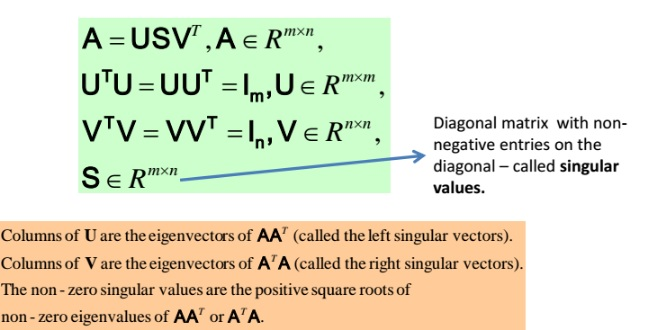
\includegraphics[width=1\linewidth, height=5cm]{Capture-4.jpg}
		\centering
		\caption{Singular Value Decomposition}
	\end{figure}\\
Given two images of a coplanar scene(image of something from different angles) taken from two different cameras, how will we determine the planar homography matrix H?How many point correspondences will we require?
    \begin{figure}[h!]
		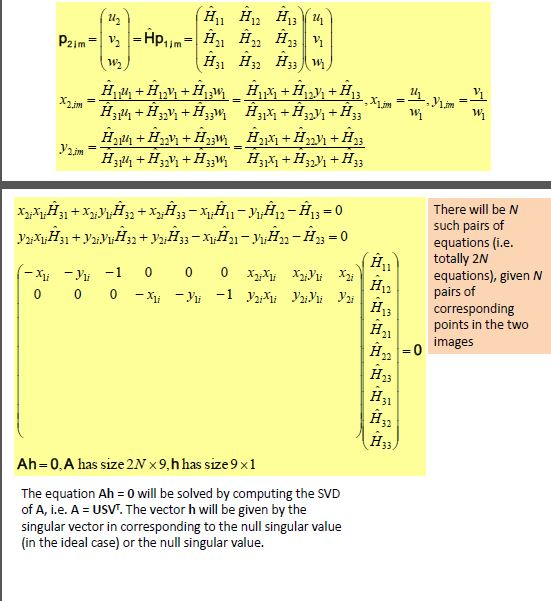
\includegraphics[width=1\linewidth, height=14cm]{Capture-1.JPG}
		\centering
		\caption{Finding Homography Matrix}
	\end{figure}\\
	
Thereafter once video is converted to orthographic projection we will use logic of video tracking specified in the  Mean\_shift\_with\_led\_and\_path.m to generate trace file as well as log file containing on and off time of LEDs.\\
The project uses the mean shift algorithm to track objects.
Mean shift is a technique to find the maxima of a density function. It is also called mode-seeking algorithm.
Mean shift finds the target using iteration and find the target that is most similar to the given target. 
In this algorithm initially a region of interest is selected, then in consecutive iterations it looks in the region of interest and shifts the mean in the direction of increasing density until no more shift is possible, i.e, it has reached the peak of the Probability Distribution Function (densest area).It would be better understood from the following figure.
    \begin{figure}[h!]
		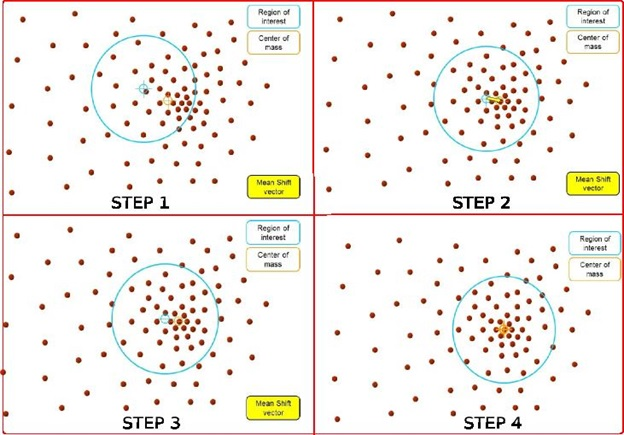
\includegraphics[width=1\linewidth, height=11cm]{ROI.jpg}
		\centering
		\caption{Illustration of Mean Shift.}
	\end{figure}\\
Robot Tracking using Mean Shift
Mean Shift Algorithm tracks objects on the basis of the feature of an object. Features can be intensity, color, gradient, etc. In the initial frame the region of interest is chosen, which is our target object. We obtain an m-bin histogram of this region after converting it to grayscale. Now PDF of each of the m bins is calculated in that region. In the next frame we again find m-bin histogram of the same region and find probability distribution of each of the m bins. Now the similarity between these bins is found out using the Bhattacharyya coefficient. To find the new target location we have to maximize the Bhattacharyya coefficient.  We move the center of the patch toward the increasing density of the Bhattacharyya coefficient. For further explanation visit\href{https://www.youtube.com/watch?v=M8B3RZVqgOo}{here} 
    \begin{figure}[h!]
		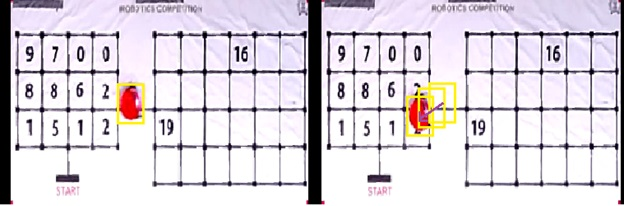
\includegraphics[width=1\linewidth, height=5cm]{ROI1.jpg}
		\centering
		\caption{Robot Tracking using Mean Shift.}
	\end{figure}\\
Detecting Glowing of Led and Determining Pick and Drop Positions
For detecting the glow of the LED we select a rectangular area around the robot and sum up number of blue pixels in each consecutive frame and subtract it with the one obtained in the previous frame. If the difference is above a certain threshold, it corresponds to LED on and a large negative value of difference below a certain threshold corresponds to LED being switched off. The number picked is then identified by mapping the position of LED glow to the original .pdf image of the arena.  

The audio processing module ampli.m is independent of the above listed processes and generates text files containing on and off time of buzzer.
We know the frequency of buzzer to near about 2.7kHz to 3kHz.We use DFT to detect this frequency and hence the buzzer beeps. Using band pass filter we filter out all the frequencies except those in this range and then output the time in a file. Choice of design of the filter and values of different parameters can be found \href{http://in.mathworks.com/help/dsp/ref/bandpassfilter.html}{here}.\\
Using the log files as input,there is C code that generates the score according to the formulae-
\begin{figure}[h!]
		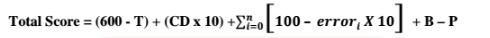
\includegraphics[width=1\linewidth, height=1cm]{score.jpg}
	\end{figure}\\
Where
\begin{itemize}
\item  error = abs(Required no- Placed no)\\ 
n can take value between 0 to 4, as there can be maximum of 4 numbers will
be present in D2.
\item T is the total time in seconds to complete the task.
\item CD is the number of correct buzzer beeps.
\item P is a penalty where 30 (thirty) points are deducted each time when LED is not turned ON or OFF correctly.
\item B is a bonus of 100 points awarded, if no error is committed.

\textbf{List of things tried during the course of project that failed-}
\end{itemize}
    \begin{tabulary}{1\textwidth}{|L|L|}
		\hline
		\textbf{Things tried} & \textbf{Reasons for failure. }\\
		\hline
		Image masking using RGB & Fixed threshold value pose a problem when lightening conditions change\\
		\hline
		Image masking using HSV & There is no particular valve of Hue or Saturation for white. \\
		\hline
		Image masking using LAB & It is the measure of degree of variation from red to green and green to yellow, so no help to identify arena, but helped us choose marker color as red. \\
		\hline
		Corner Detection using Harris Corner & Does not always give us exact four corners.\\
		\hline
		Corner Detection using vector dot product & The edges that are masked are not smooth enough.\\
		\hline
		Corner Detection using polar co-ordiantes & Since many videos did not have all corners visible. \\
		\hline
		Path following by providing equations & All the equations needed to be provided manually \\
		\hline
		Path following by providing specific path by drawing path & There may be more than one correct path and drawing each is not possible\\
		\hline
		LED detection by Hue and RGB values & Since arena was white and glowing LED would not change the pixel intensity to the extent that it could be detected.\\
		\hline
		LED detection by difference in intensity values & Since different parts of arena had different lightening conditions, their intensity values changed without the LED glowing.\\
		\hline
		Audio Detection By Amplitude & Affected too much by noise.\\
		\hline		
	\end{tabulary}\\
	
\section{Use and Demo}
\textbf{Final Setup Image.}
    \begin{figure}[h!]
		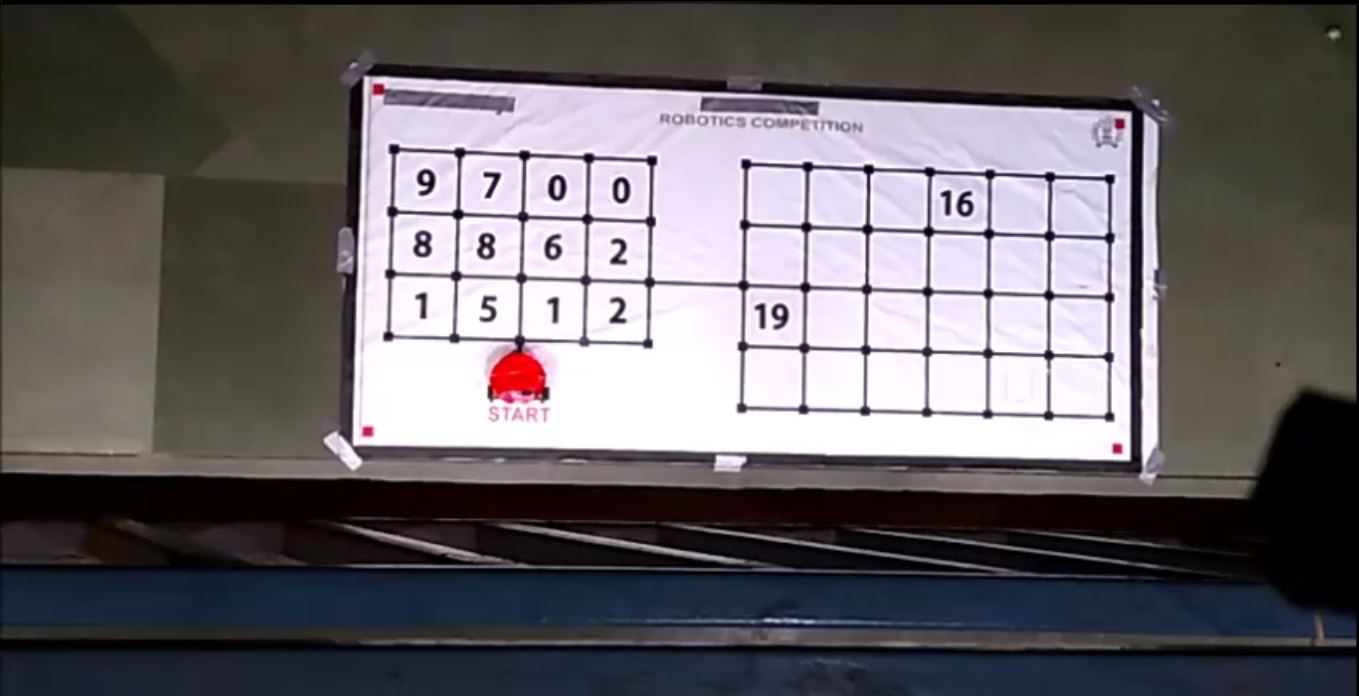
\includegraphics[width=1\linewidth, height=8cm]{Capture.JPG}
		\centering
		\caption{Testing Purpose}
	\end{figure}\\
\textbf{User Instruction for demonstration}
\begin{itemize}
  \item The position of the arena should be as shown with all the corners visible.
  \item 4cm thick black chart paper must be pasted on the borders of the arena.
  \item Four 2cmx2cm red markers need to be pasted on four corners.
  \item Camera should be entirely stable without any movement and it should be above directly above the arena.
  \item Adequate lightening must be present and there should not be much variation in conditions during filming the video.
  \item The robot should be covered with red colored paper as shown in the image.
\end{itemize}
\textbf{Demonstration Videos}\\
\href{https://youtu.be/vaqDc_Qd9p8}{Original video with theme implemented.}\\
\href{https://youtu.be/ZgN-Ncc9VRw}{Part of the original video that is being processed.}\\
\href{https://youtu.be/vI5nk7CcUwI}{Homographed Video of task.}\\
\href{https://youtu.be/gpSy3z4Rkdc}{Object tracking implemented on the video.}

\section{Future Work}
\begin{itemize}
\item First of all we need to implement parallel processing in our code since the time for evaluation is humongous to be of any practical use.
Parallel processing is useful when previous outputs do not affect the present inputs.\\
Here we know each frame is represented as matrix and to transform it to orthographic projection we perform operations on each point of the matrix.Now each point is independent to any other point in matrix and operations on them can be done parallely via GPU.
\item Secondly relying just on image processing is not going to allow us achieve our goal of making this evaluation generic. We can incorporate machine learning as well.Machine learning helps computers to learn without being explicitly programmed. It focuses on the development of computer programs that can teach themselves to grow and change when exposed to new data.\\
We can use concepts of ML to identify the arena, the robot and even to identify a perfect run(i.e by giving it samples of prefect task completion).
\end{itemize}

\section{Bug report and Challenges}
\begin{itemize}
\begin{figure}[h!]
		\begin{subfigure}{0.4\textwidth}
		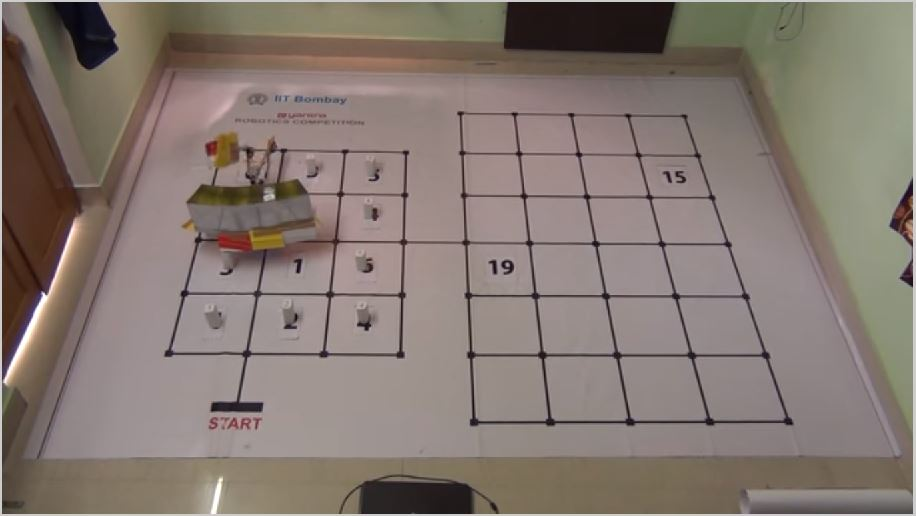
\includegraphics[width=1\linewidth, height=2cm]{1.JPG}
			\caption{Earlier}
		\end{subfigure}
		\begin{subfigure}{0.4\textwidth}
			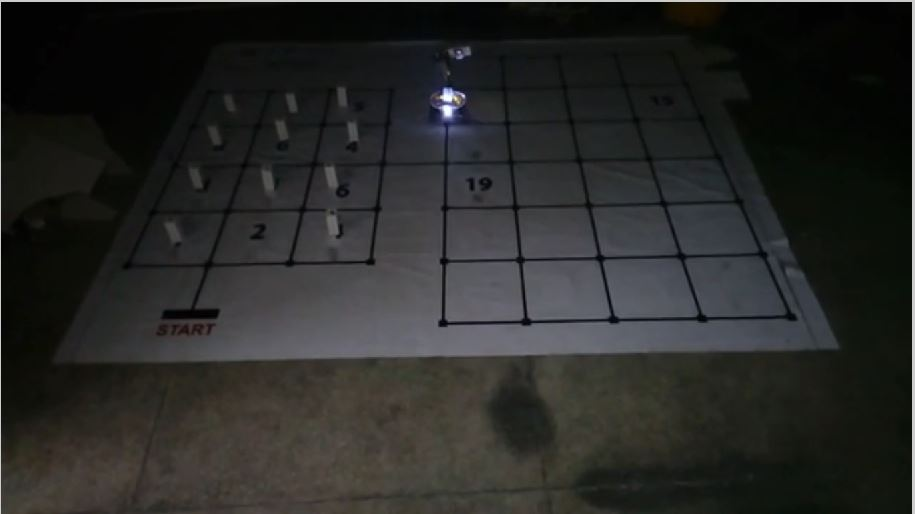
\includegraphics[width=1\linewidth, height=2cm]{3.JPG}
			\caption{Later}
		\end{subfigure}
	\end{figure}	
	 \begin{figure}[h!]
		\begin{subfigure}{0.4\textwidth}
			
\includegraphics[width=1\linewidth, height=2cm]{11.JPG}
			\caption{Thresholding earlier image}
		\end{subfigure}
		\begin{subfigure}{0.4\textwidth}
			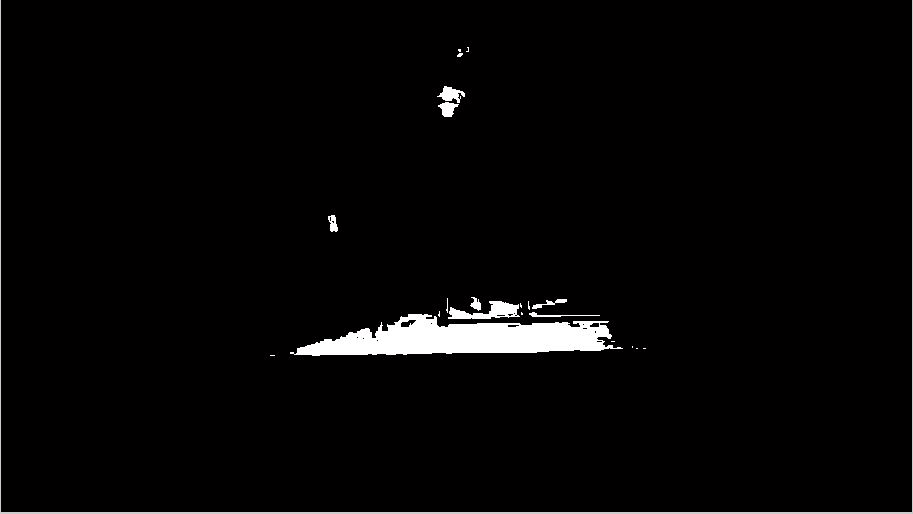
\includegraphics[width=1\linewidth, height=2cm]{33.JPG}
			\caption{Thresholding later with same threshold values}
		\end{subfigure}
	\end{figure}
    \item Change in lightening condition during videos pose an large risk of error generation.Errors such as incorrect detection of robot, improper detection of the area of the arena. These errors occur because we have taken RGB colorspace to threshold the image and detect various objects and these thresholding values are very sensitive to lightening conditions.
	\item The audio processing module isn't accurate. The manually set threshold works in about 70\% of the cases.Rest of the time minor changes in thresholding needs to be done to get desired result.
    \item Another problem with the code is that the homography part isn't optimized. The pre-processing time is too much to be of any practical use,since video of about a minute and half takes nearly 20 minutes to convert. 
\end{itemize}




\begin{thebibliography}{li}
\bibitem{wavelan97}
Dr. Niket Kaisare
{\em \href{https://www.youtube.com/watch?v=pj4KKLUMIAg&list=PLa8a_8vztYc7aK6H4bpQTbOqelVIND9Aw}{Introduction to Matlab}}.
\bibitem{wavelan97}
Dorin Comaniciu, Visvanathan Ramesh, Peter Meer
{\em \href{http://comaniciu.net/Papers/MsTracking.pdf}{Research paper on mean shift}}.
\bibitem{wavelan97}
 Rashi Agrawal
{\em \href{https://www.youtube.com/watch?v=-cSVGwAwZZ4&list=PLEo-jHOqGNyUWoCSD3l3V-FjX9PnHvx5n}{Introduction to DIP using Matlab}}.
\bibitem{wavelan97}
 Dr. Mubarak Shah
{\em \href{https://www.youtube.com/watch?v=M8B3RZVqgOo}{UCF Computer Vision Video Lectures}},
2012.
\bibitem{wavelan97}
Mathworks Community
{\em \href{http://in.mathworks.com/help/signal/examples/practical-introduction-to-frequency-domain-analysis.html}{Audio Processing.}}
\bibitem{wavelan97}
Wikipedia
{\em \href{https://en.wikipedia.org/wiki/Support_vector_machine}{Support Vector Machine.}}

\end{thebibliography}


\end{document}

